\documentclass[a4paper]{report}

% \usepackage[utf8]{inputenc}
% \usepackage[T1]{fontenc}
% \usepackage{textcomp}
\usepackage[english]{babel}
\usepackage{amsmath, amssymb}
\usepackage[separate-uncertainty=true, multi-part-units=single]{siunitx}
\usepackage[]{subfig}
\usepackage[colorlinks=true, anchorcolor=blue, linkcolor=blue, citecolor=blue, bookmarks=false,hyperfootnotes=false]{hyperref}
\usepackage[margin=1in]{geometry}
\usepackage{color,soul}
\usepackage{tabularx}

% figure support
\usepackage{import}
\usepackage{xifthen}
\pdfminorversion=7
\usepackage{pdfpages}
\usepackage{transparent}
\usepackage{physics}
\graphicspath{ {./figures/} }
% \setlength{\parindent}{0pt}
\usepackage{chngcntr}
\usepackage{verbatim}
\usepackage{indentfirst}
\numberwithin{equation}{section}
\counterwithin{figure}{section}
\newcommand{\incfig}[1]{%
		\def\svgwidth{\columnwidth}
		\import{./figures/}{#1.pdf_tex}

}

\pdfsuppresswarningpagegroup=1

% for citations / references
\usepackage[style=ieee]{biblatex}
\addbibresource{moess_report.bib}

\begin{document}

%----------------------------------------------------------------------------------------
%	TITLE PAGE
%----------------------------------------------------------------------------------------
\begin{titlepage} % Suppresses displaying the page number on the title page and the subsequent page counts as page 1
	\newcommand{\HRule}{\rule{\linewidth}{0.5mm}} % Defines a new command for horizontal lines, change thickness here
	
	\center % Centre everything on the page
	%------------------------------------------------
	%	Headings
	%------------------------------------------------
	
	\textsc{\LARGE Rheinische Friedrich-Wilhelms-Universit\"at Bonn }\\[4cm] % Main heading such as the name of your university/college
	
	\textsc{\Large Advanced Laboratory Course}\\[0.5cm] % Major heading such as course name
	
	\textsc{\large Performed on: April 22, 2022}\\[0.5cm] % Minor heading such as course title

	\textsc{\large Submitted on: May 13, 2022}\\[0.5cm] % Minor heading such as course title
	
	%------------------------------------------------
	%	Title
	%------------------------------------------------
	
	\HRule\\[0.4cm]
	
	{\huge\bfseries K221: M{\"{o}}{\ss}bauer Effect}\\[0.4cm] % Title of your document
	
	\HRule\\[1.5cm]
	
	%------------------------------------------------
	%	Author(s)
	%------------------------------------------------
	
	\begin{minipage}{0.4\textwidth}
		\begin{flushleft}
			\large
			\textit{Authors}\\
			Paarth Thakkar \\
			Keito Watanabe
		\end{flushleft}
	\end{minipage}
	~
	\begin{minipage}{0.4\textwidth}
		\begin{flushright}
			\large
			\textit{Tutor(s)}\\
			Dr. Jens Barth
		\end{flushright}
	\end{minipage}

	\vspace*{5em}

	\begin{minipage}{0.8\textwidth}
		\begin{centering}
			% \large
			\textbf{Abstract}\\[0.2cm]

		\end{centering}
	\end{minipage}
	
	% If you don't want a supervisor, uncomment the two lines below and comment the code above
	%{\large\textit{Author}}\\
	%John \textsc{Smith} % Your name
	
	%------------------------------------------------
	%	Date
	%------------------------------------------------
	
	%\vfill\vfill\vfill % Position the date 3/4 down the remaining page
	% \vfill\vfill
	
	% {\large\today} % Date, change the \today to a set date if you want to be precise
	
	%------------------------------------------------
	%	Logo
	%------------------------------------------------
	
	%\vfill\vfill
	%\includegraphics[width=0.2\textwidth]{placeholder.jpg}\\[1cm] % Include a department/university logo - this will require the graphicx package
	 
	%----------------------------------------------------------------------------------------
	
	% \vfill % Push the date up 1/4 of the remaining page
	
\end{titlepage}



\tableofcontents

\chapter{Introduction}


\chapter{Theory}

\chapter{Experimental Set-Up and Procedure}

\section{Experimental Set-Up}

To measure the Moessbauer spectrum, we placed a Co-57 radioactive source onto a table with a moving absorber 
that has a maximum displacement of $\SI[]{25.1 \pm 0.2}[]{\milli\metre}$.  A photodetector is placed 
behind the absorber that detects the number of photons that are not absorbed via this process. The speed of the 
absorber is controlled by a motor that uses the voltage as an input. See Fig. \ref{apparatus_source}
for the Moessbauer source apparatus. \par 

\begin{figure*}[htb!]
	\centering
	\includegraphics[width=0.7\columnwidth]{source_image.png}

	\caption{The set-up of the Moessbauer source. \textit{Left}: The Co-57 source. \textit{Middle}: 
	The moving absorber. \textit{Right}: The photodetector which is connected to the detector apparatus.
	}
	\label{fig:apparatus_source}
\end{figure*}

The photodetector is then connected to a single channel analyzer (SCA), which determines the number of counts detected
in a given time range and maximal and minimal width to observe the counts. The SCA has 2 main parameters that should be modified:
the Upper Level Discrimator (ULD) and the Lower Level Discrimator (LLD), which controls the binsize and the lower limit for 
photodetection respectively. The modes of the ULD can be set to measure with a higher resolution by detecting counts with 
10 $\%$ of the binsize. The SCA was then connected to a display in which the number of counts obtained in a specific time 
interval was shown. 
The photodetecting apparatus consisted of two such setups to consider for measurements with positive and negative velocity 
of the absorber as the offset voltage between the two can allow the measurements in the LR and RL direction to differ.
 A separate run counter that tracks the number of turns that the absorber had is also contained in the apparatus. A timer 
 that controls the time interval of measurement is also placed which is used for the calibration process.
See Fig. \ref{fig:apparatus_raw} for the apparatus used for the photodetection as well as the schematic of the apparatus. \par 

\begin{figure*}[htb!]
	\centering
	\subfloat[]{{\includegraphics[width=0.45\columnwidth]{apparatus_image.png}}}
	\quad
	\centering
	\subfloat[]{{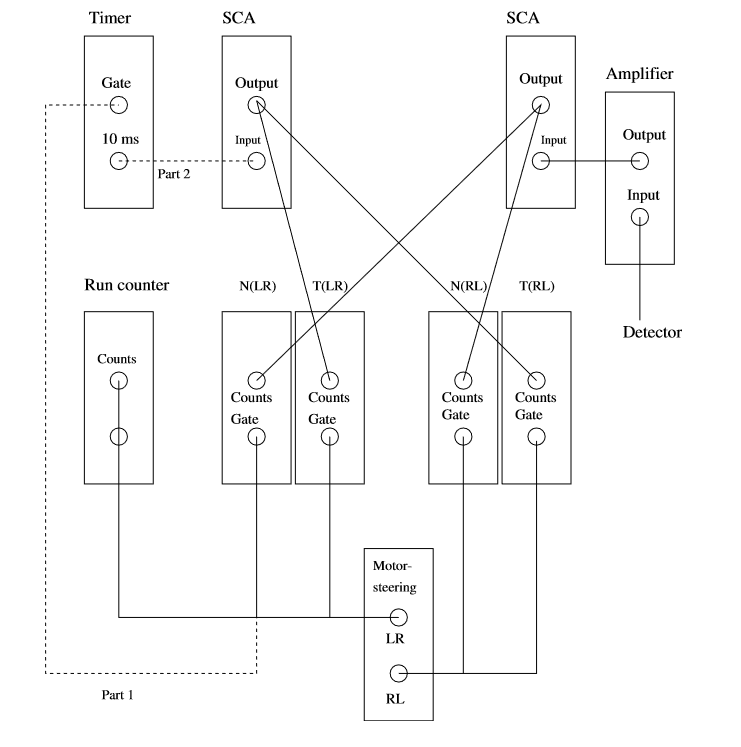
\includegraphics[width=0.45\columnwidth]{apparatus_schematic.png}}}
	\caption{(a) The photodetector apparatus used in this experiment. (b) The schematic of the apparatus. Obtained from 
			Ref. \cite{k2212016}.}
	\label{fig:apparatus_raw}
\end{figure*}

\section{Procedure}

\subsection{Calibration of SCA}

Before we took any measurements, we determined the optimal values for the LLD in order to ensure that we are 
detecting counts from the 14.4 keV transition. In order to do so, we modified the LLD from 0 to 4 and determined the number 
of counts obtained at each value. The ULD and time interval was fixed to be 10 for all measurements. Once the data was obtained, 
we plotted the count rate $N / T$ against the LLD values and compared our results to the Fe-57 $\gamma$-spectrum as seen in Fig. \hl{add reference here}.
Fig. \ref{fig:calib_plot} shows the obtained spectrum from our experiment.

% \begin{figure*}[htb!]
% 	\centering
% 	\includegraphics[width=0.7\columnwidth]{source_image.png}

% 	\caption{The set-up of the Moessbauer source. \textit{Left}: The Co-57 source. \textit{Middle}: 
% 	The moving absorber. \textit{Right}: The photodetector which is connected to the detector apparatus.
% 	}
% 	\label{fig:calib_plot}
% \end{figure*}

We identified the 14.4 keV transition line as the third peak on Fig. . 

\chapter{Results and Discussion}

\chapter{Conclusion and Outlook}

\chapter{Acknowledgements}

\printbibliography

\chapter{Appendix}


\end{document}